\subsection*{Modello 3 - medium-200-0}

% Introduzione su strategia del training -> qual è l'obiettivo dell'esperimento?
L'idea per l'esperimento successivo è stata quella di utilizzare un modello con più parametri e
pertanto optare per una dimensione di YOLO più grande, nello specifico la dimensione media YOLOv8m. 
Se è vero che il numero di epoche rimane
alto, dall'altra parte si spera di poter raggiungere prestazioni migliori con una rete più profonda.

Il numero di epoche è stato impostato a 200 perché vedendo il precedente tentativo con il modello small
ci aspettavamo quel tanto di epoche prima che il modello iniziasse a overfittare i dati. 

Nella tabella \ref{tab:v3-model-configs} sono riportati gli iperparametri di questo esperimento. 
Rispetto al modello \texttt{small-1203} non ci sono particolari differenze se non il numero di epoche e 
la dimensione del modello di YOLO. 

\begin{table}[!htb]
    \centering
    \begin{tabular}{lc}
        \hline
        \textbf{Iperparametro} & \textbf{Valore} \\
        \hline
        epoche & 200  \\
        optimizer & auto (SGD) \\
        learning rate (lr0) & 0.01 \\
        learning rate (lrf) & 0.01 \\
        momentum & 0.937 \\
        weight\_decay & 0.0005 \\
        imgsz & 640 \\
        dropout & 0.15 \\
        patience & 100 \\
        \midrule
        hsv\_h & 0.7 \\
        degrees & 120 \\
        shear & 55 \\
        \hline
    \end{tabular}
    \caption{Configurazione iperparametri del modello \texttt{medium-200-0} per il training}
    \label{tab:v3-model-configs}
    \end{table}

    
    % Dettagli configurazione, tipologia modello e iperparametri, dove è stato eseguito il train

% Risultati training
% - andamento training

\begin{figure}[!htb]
    \centering
    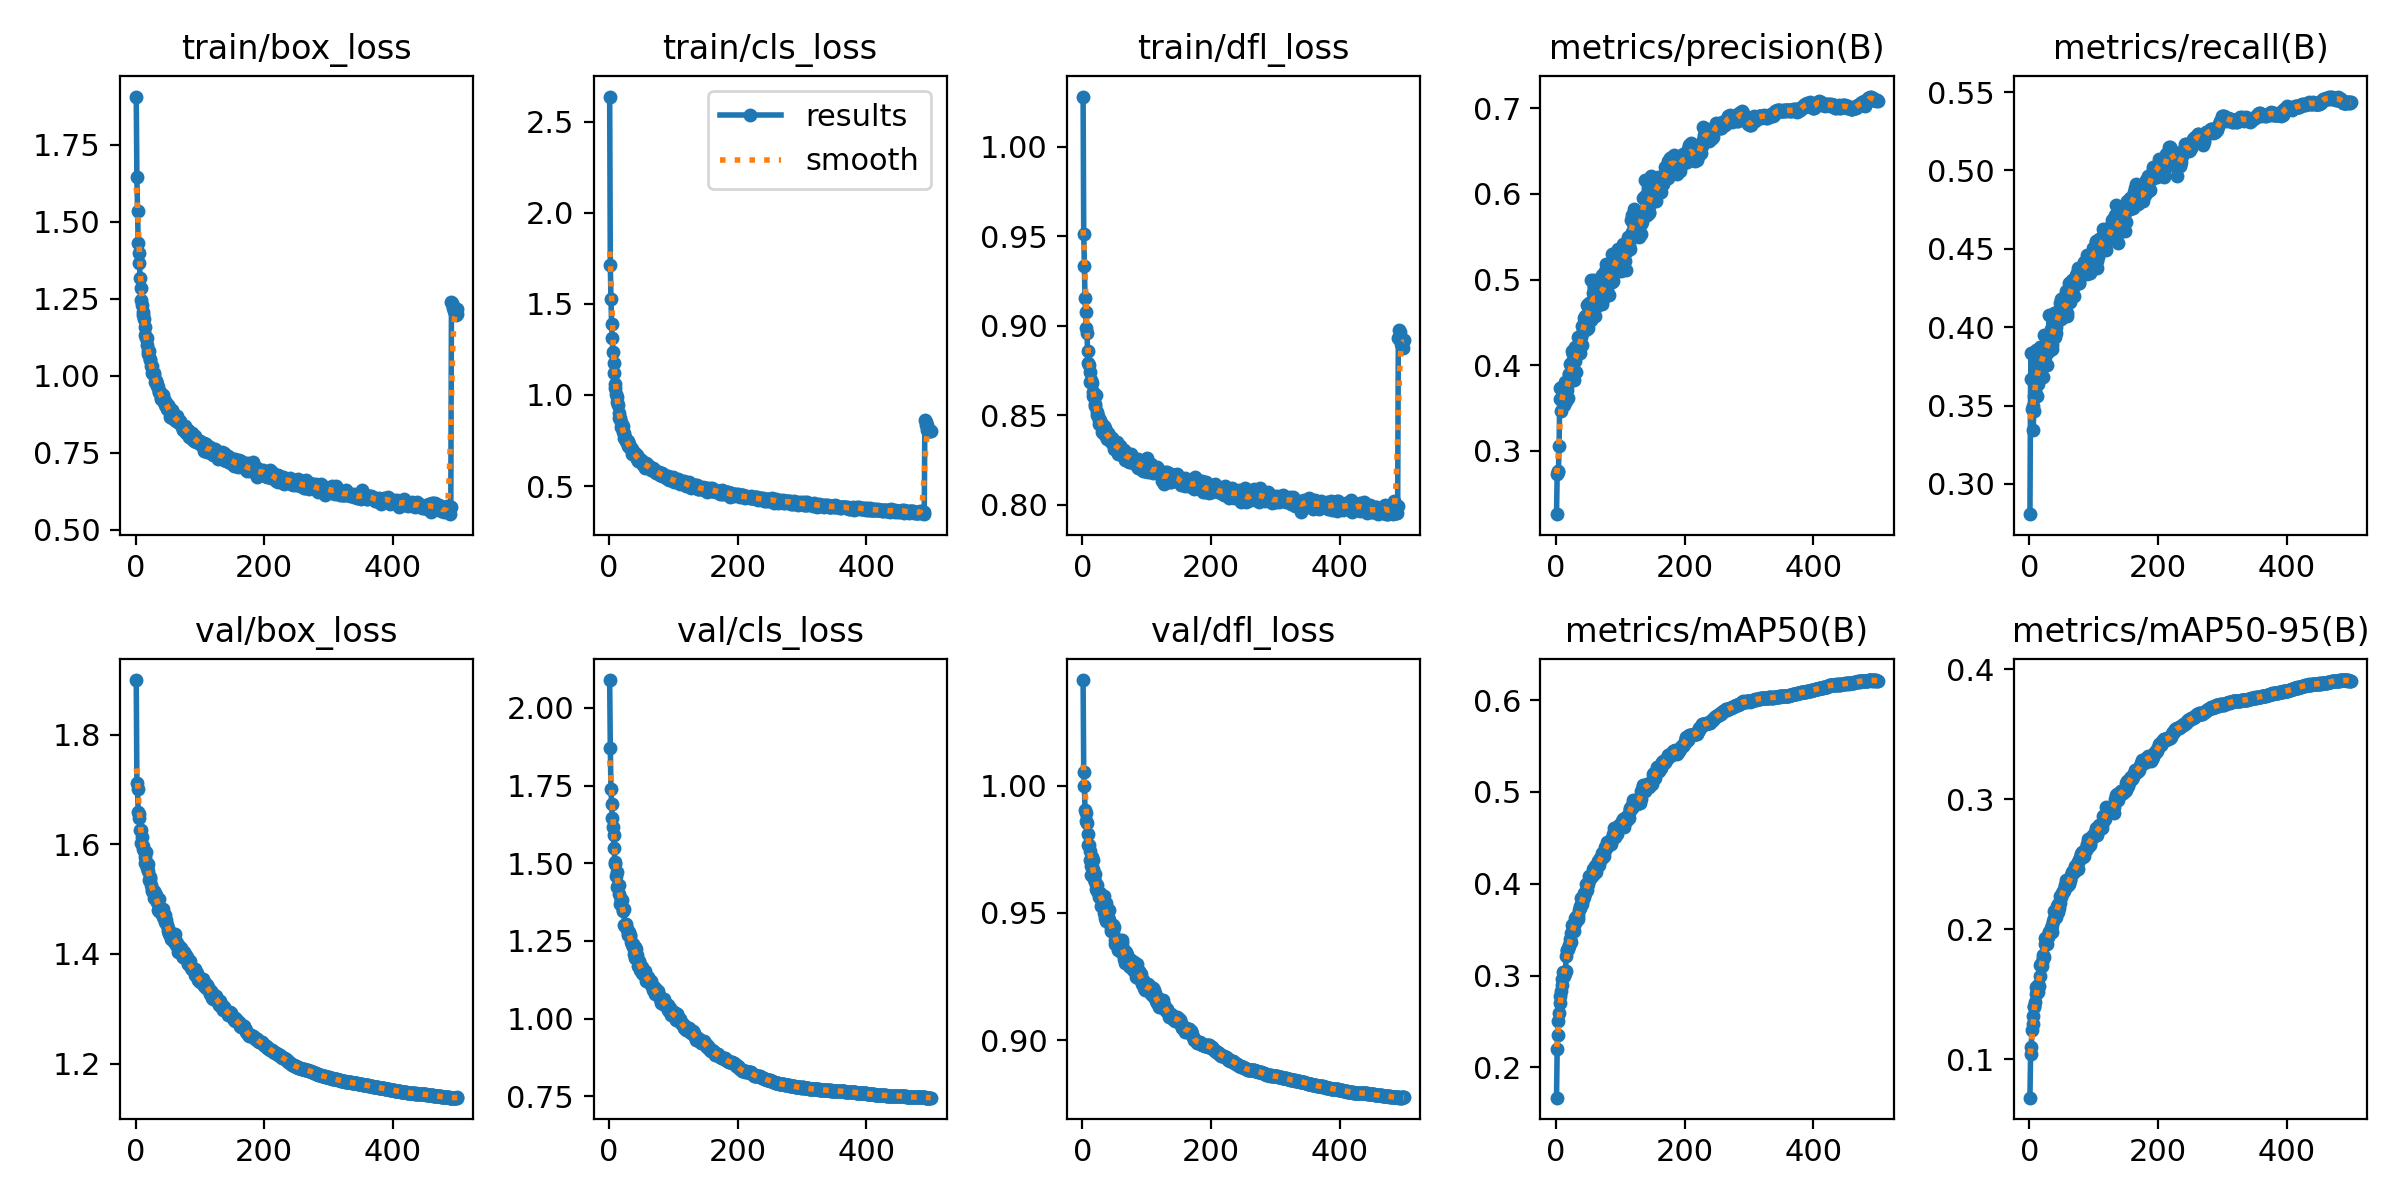
\includegraphics[width=0.8\textwidth]{v_3/results.png}
        \caption{Andamento funzioni di loss e metriche durante l'esecuzione di \texttt{medium-200-0}}
        \label{fig:v3-2}
    \end{figure}
    % - grafici recall e precision e performance e F1
    \begin{figure}[!htb]
        \centering
        \begin{subfigure}{.5\textwidth}
            \centering
            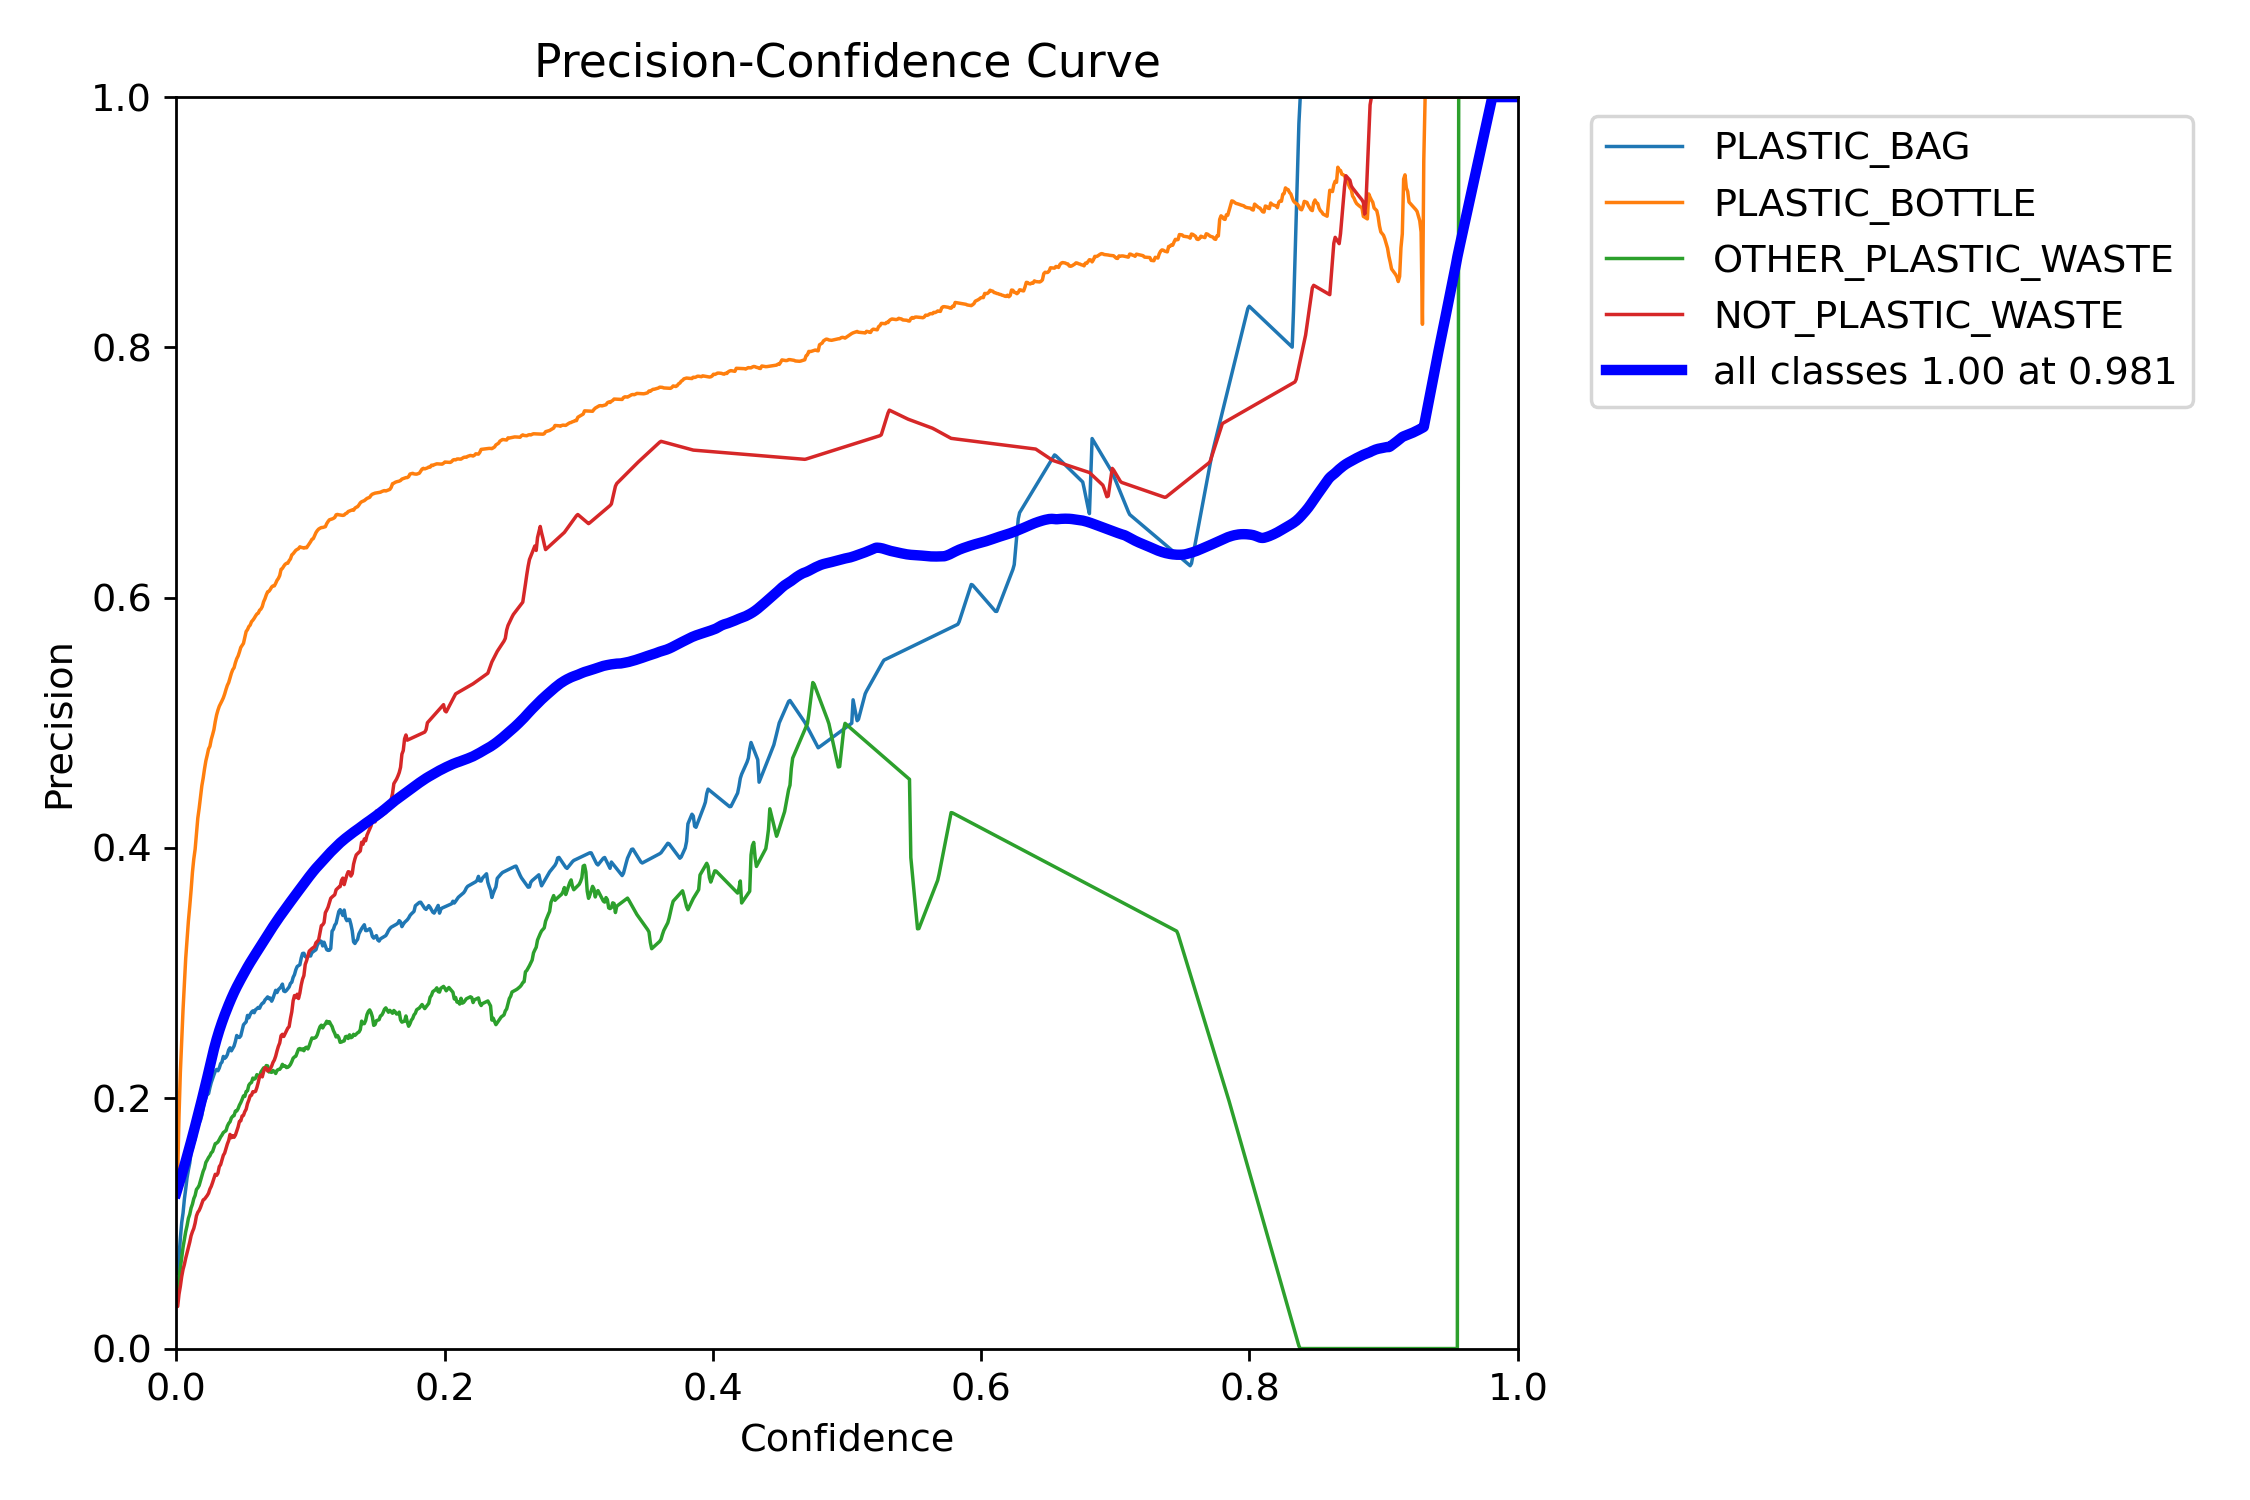
\includegraphics[width=.9\linewidth]{v_3/P_curve.png}
            \subcaption{P-curve}
            \label{fig:v3-3.1}
        \end{subfigure}%
          \begin{subfigure}{.5\textwidth}
            \centering
            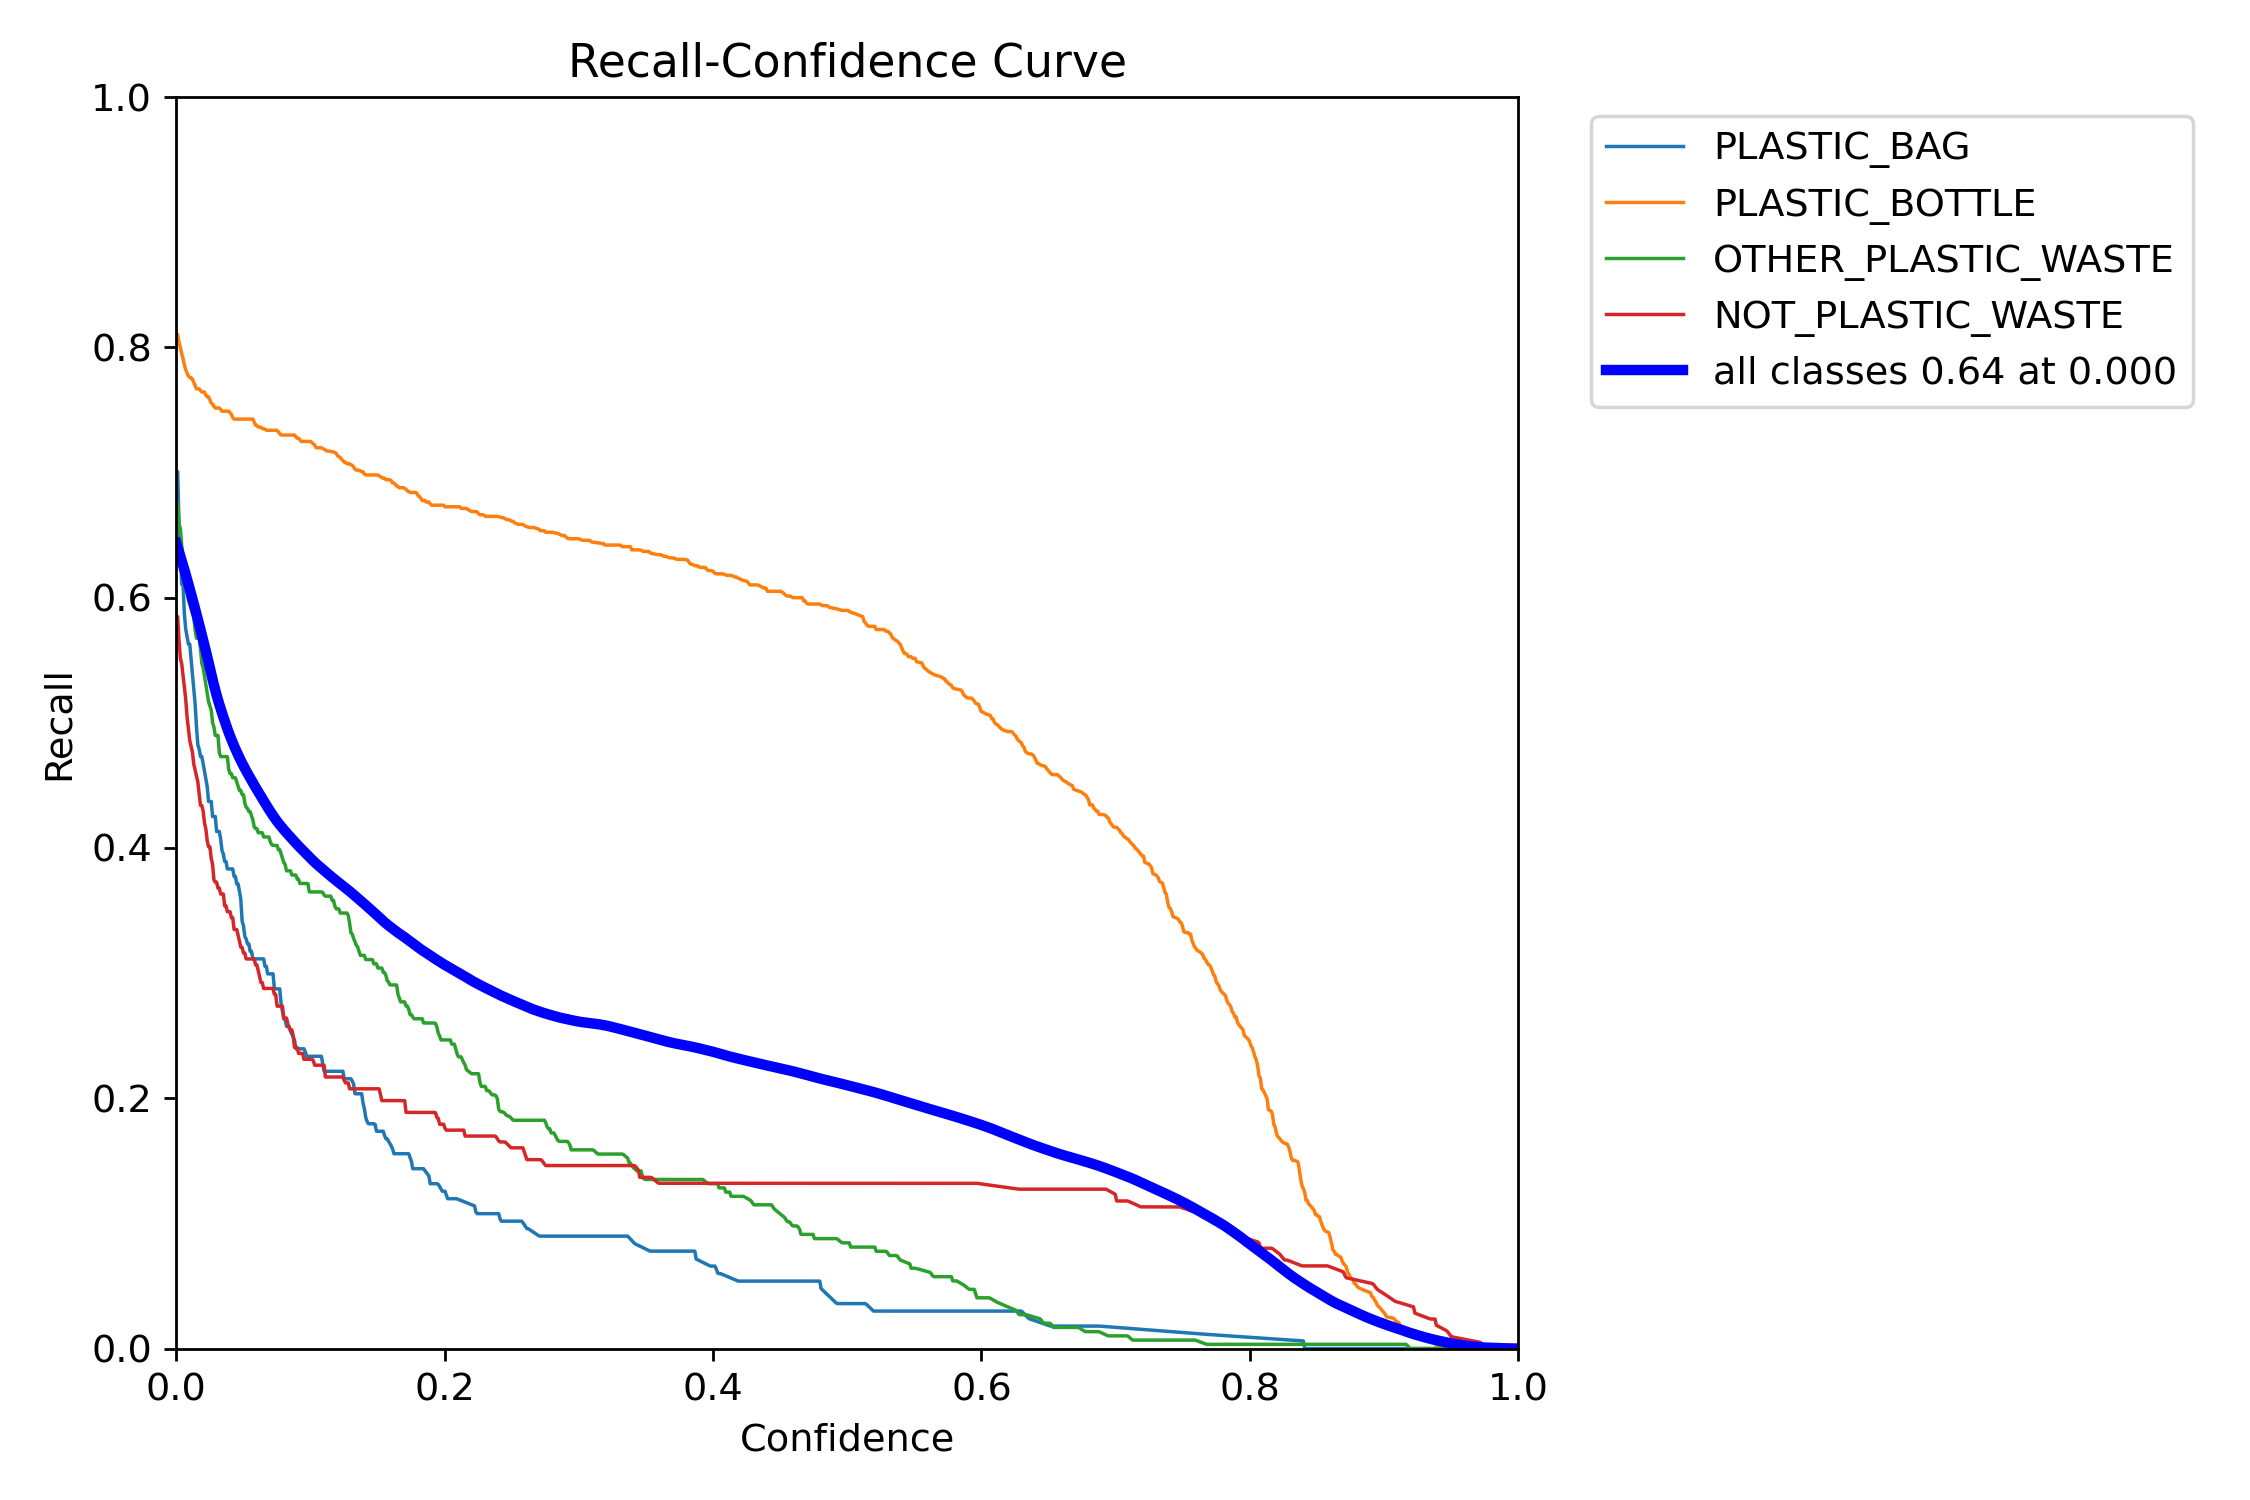
\includegraphics[width=.9\linewidth]{v_3/R_curve.png}
            \subcaption{R-curve}
            \label{fig:v3-3.2}
        \end{subfigure}
        \vskip\baselineskip
        \begin{subfigure}{.5\textwidth}
            \centering
            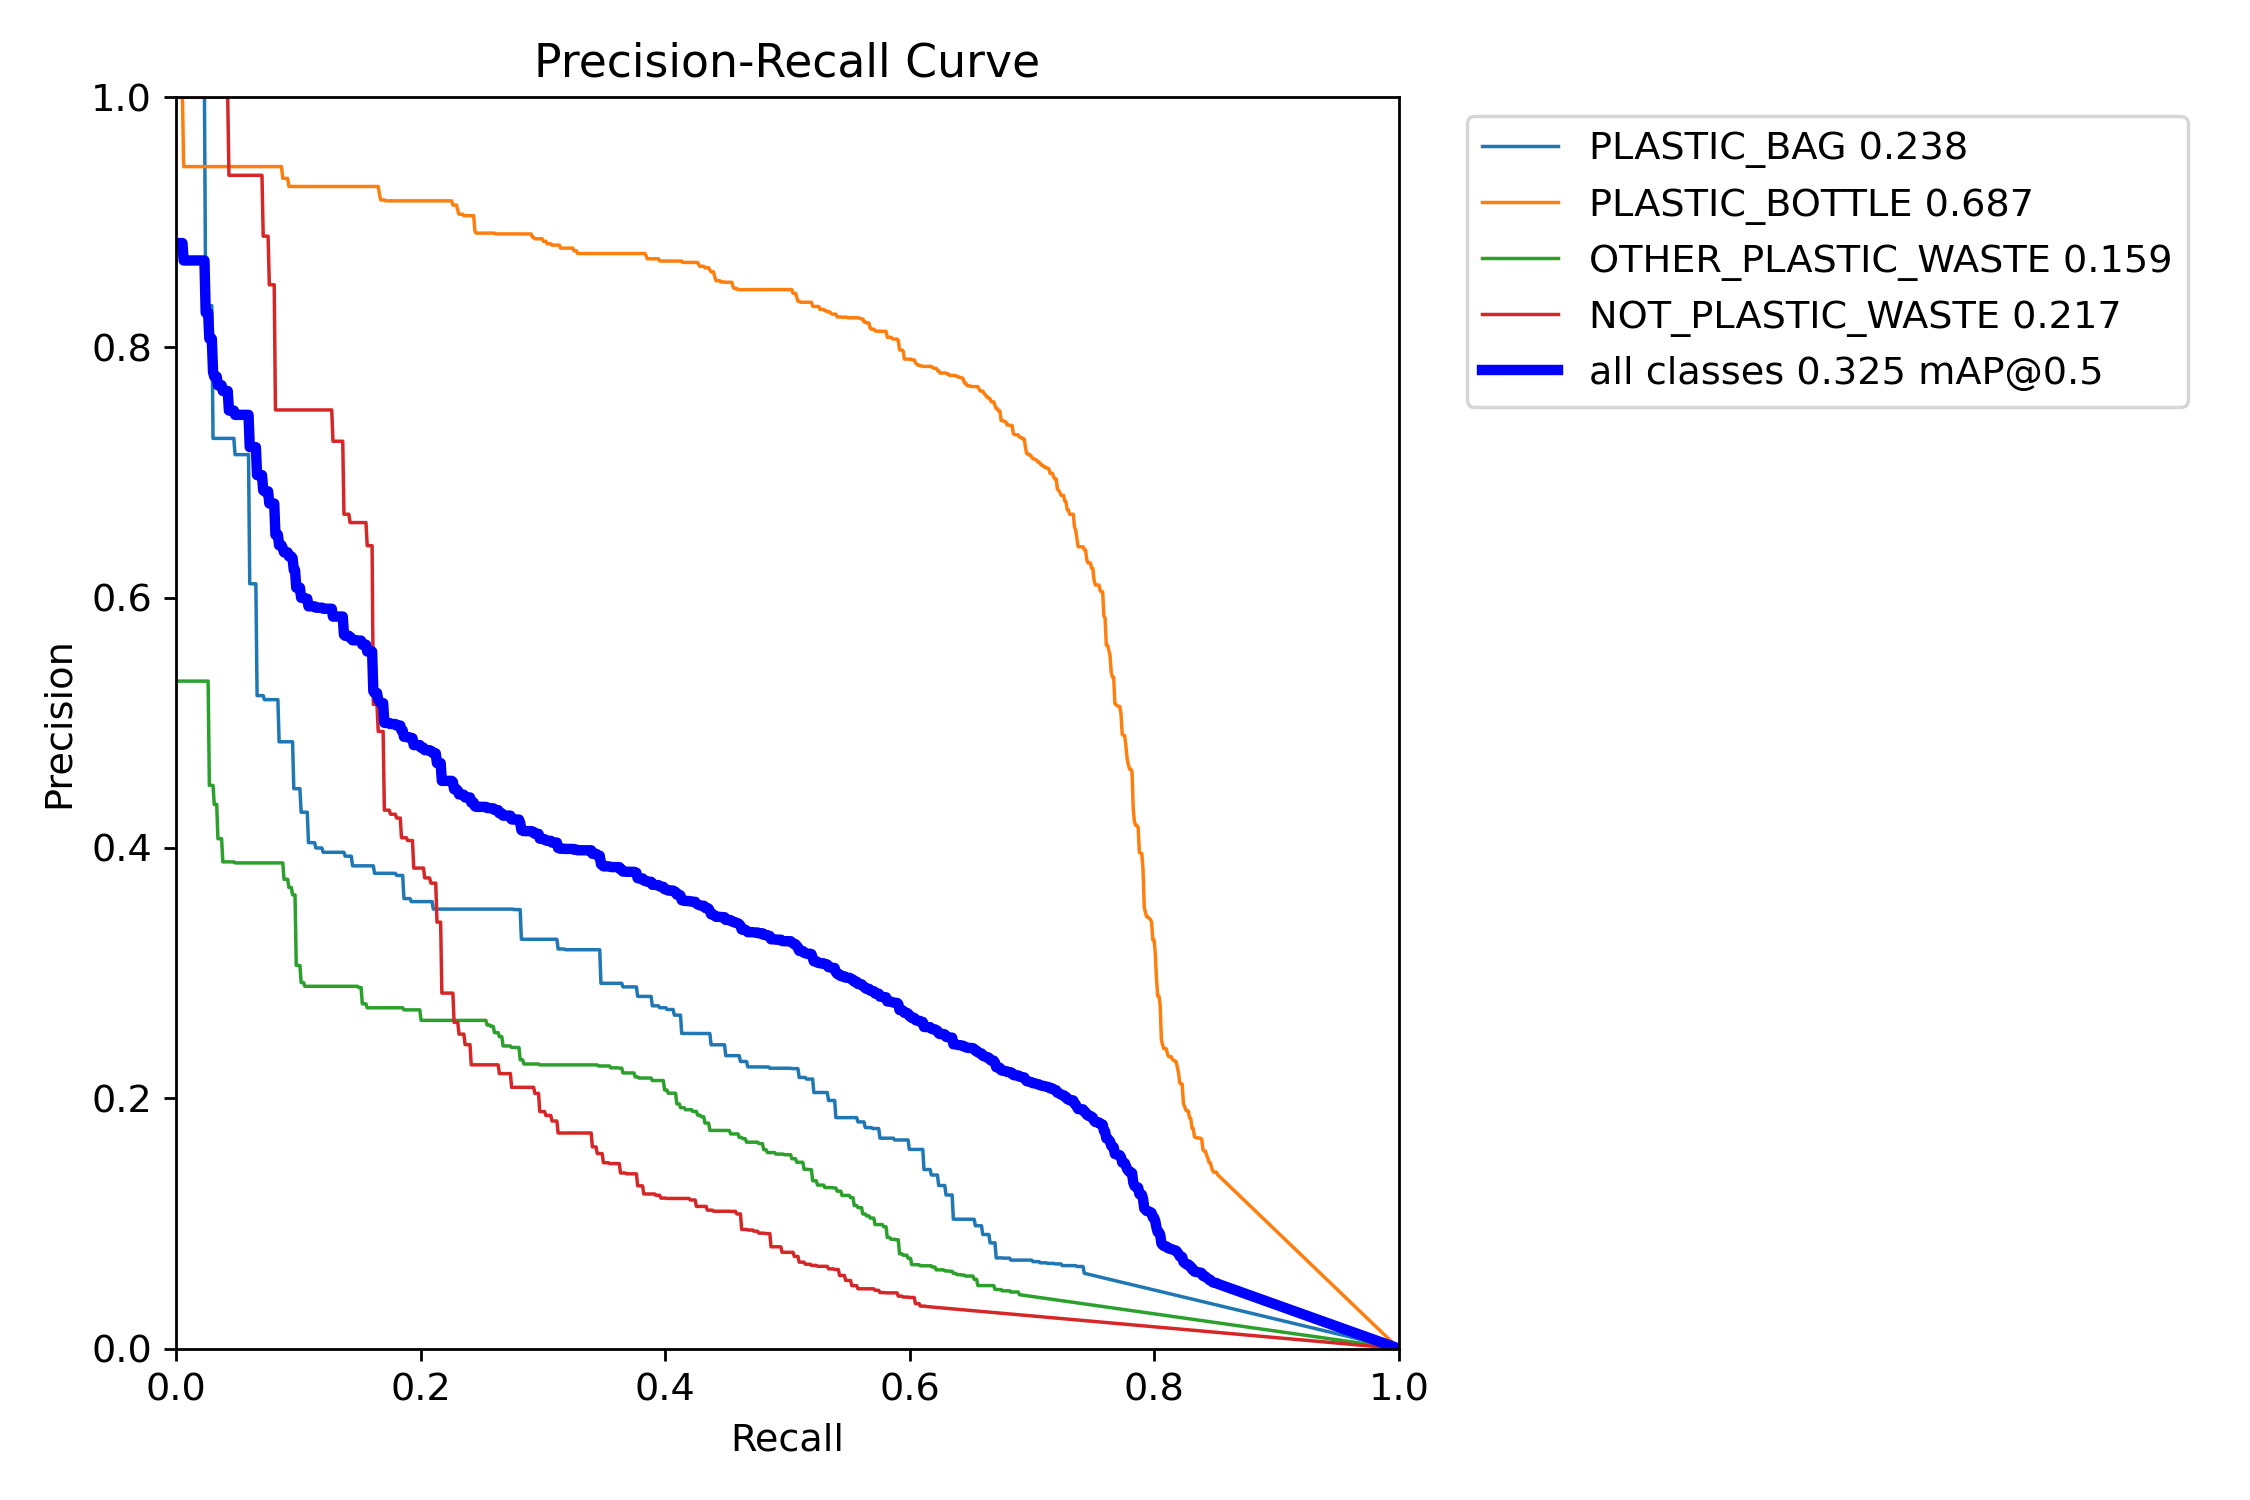
\includegraphics[width=.9\linewidth]{v_3/PR_curve.png}
            \subcaption{PR-curve}
            \label{fig:v3-3.3}
        \end{subfigure}
        \begin{subfigure}{.49\textwidth}
            \centering
            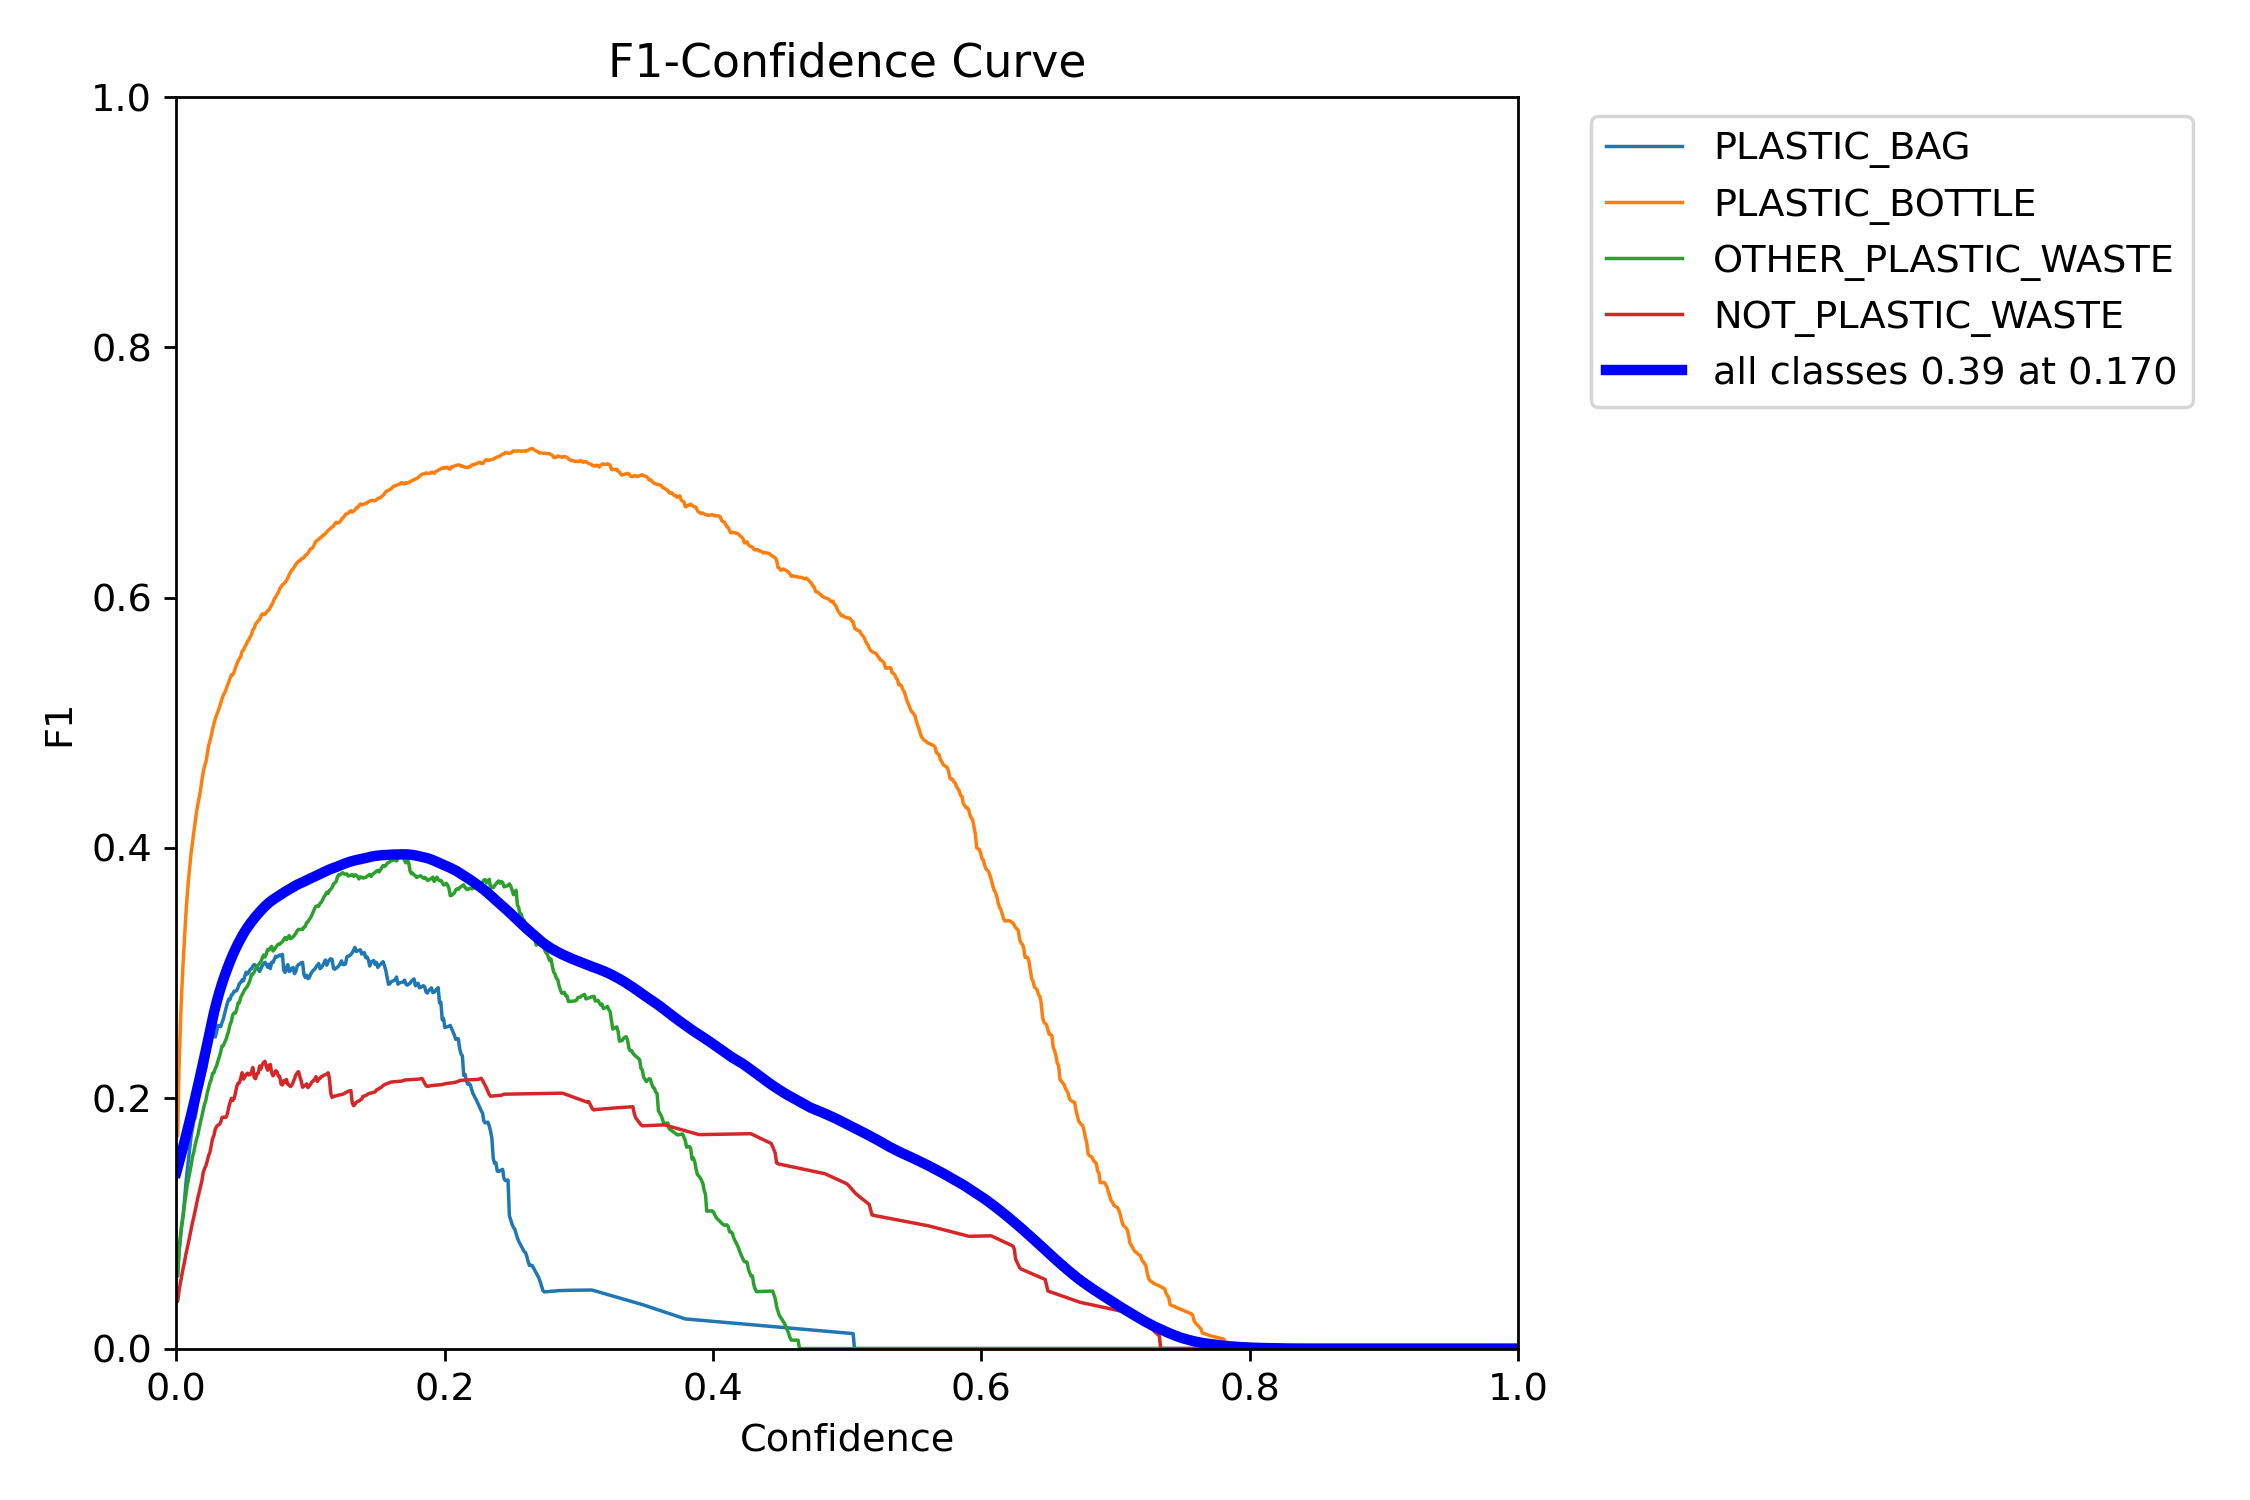
\includegraphics[width=.9\linewidth]{v_3/F1_curve.png}
            \subcaption{F1-curve}
            \label{fig:v3-3.4}
        \end{subfigure}
        
        \caption{Andamento funzioni di loss e metriche durante l'esecuzione di \texttt{medium-200-0}}
        \label{fig:v3-3}
    \end{figure}
    
    La fase di addrestramento è stata eseguita su server Google colab sfruttando le GPU T4 a disposizione, 
    esattamente come è stato per gli esperimenti precedenti.
    
    I risultati ottenuti sono simili e leggermente migliori rispetto a quelli ricavati dai modelli 
    più piccoli. Si è raggiunto un valore discreto di mAP pari a 39.1\% mentre tutte le problematiche 
    dovute alla distribuzione sbilanciata delle istanze rimangono. 

In genere il modello tende a riconoscere per lo più bottiglie di plastica e a confondere tra loro
in alcuni casi le altre classi. Tali problematiche hanno portato a cercare altre soluzioni con
l'obiettivo di migliorare i risultati finora raggiunti.

    \begin{table}[!htb]
        \centering
        \begin{tabularx}{\textwidth}{lYYYc}
            \toprule
            Class & P & R & mAP50 & mAP50-95 \\
            \midrule
            ALL & 0.456 & 0.459 & 0.391 & 0.186 \\
            PLASTIC\_BAG & 0.483 & 0.482 & 0.384 & 0.142 \\
            PLASTIC\_BOTTLE & 0.756 & 0.712 & 0.744 & 0.374 \\
            OTHER\_PLASTIC\_WASTE & 0.150 & 0.361 & 0.131 & 0.0483 \\
            NOT\_PLASTIC\_WASTE & 0.435 & 0.279 & 0.305 & 0.178 \\
            \bottomrule
        \end{tabularx}
        \caption{Risultati delle metriche sul test set per \texttt{medium-200-0}}
        \label{table:v3-1}
    \end{table}

    % - matrici di confusione
    \begin{figure}[!htb]
        \centering
        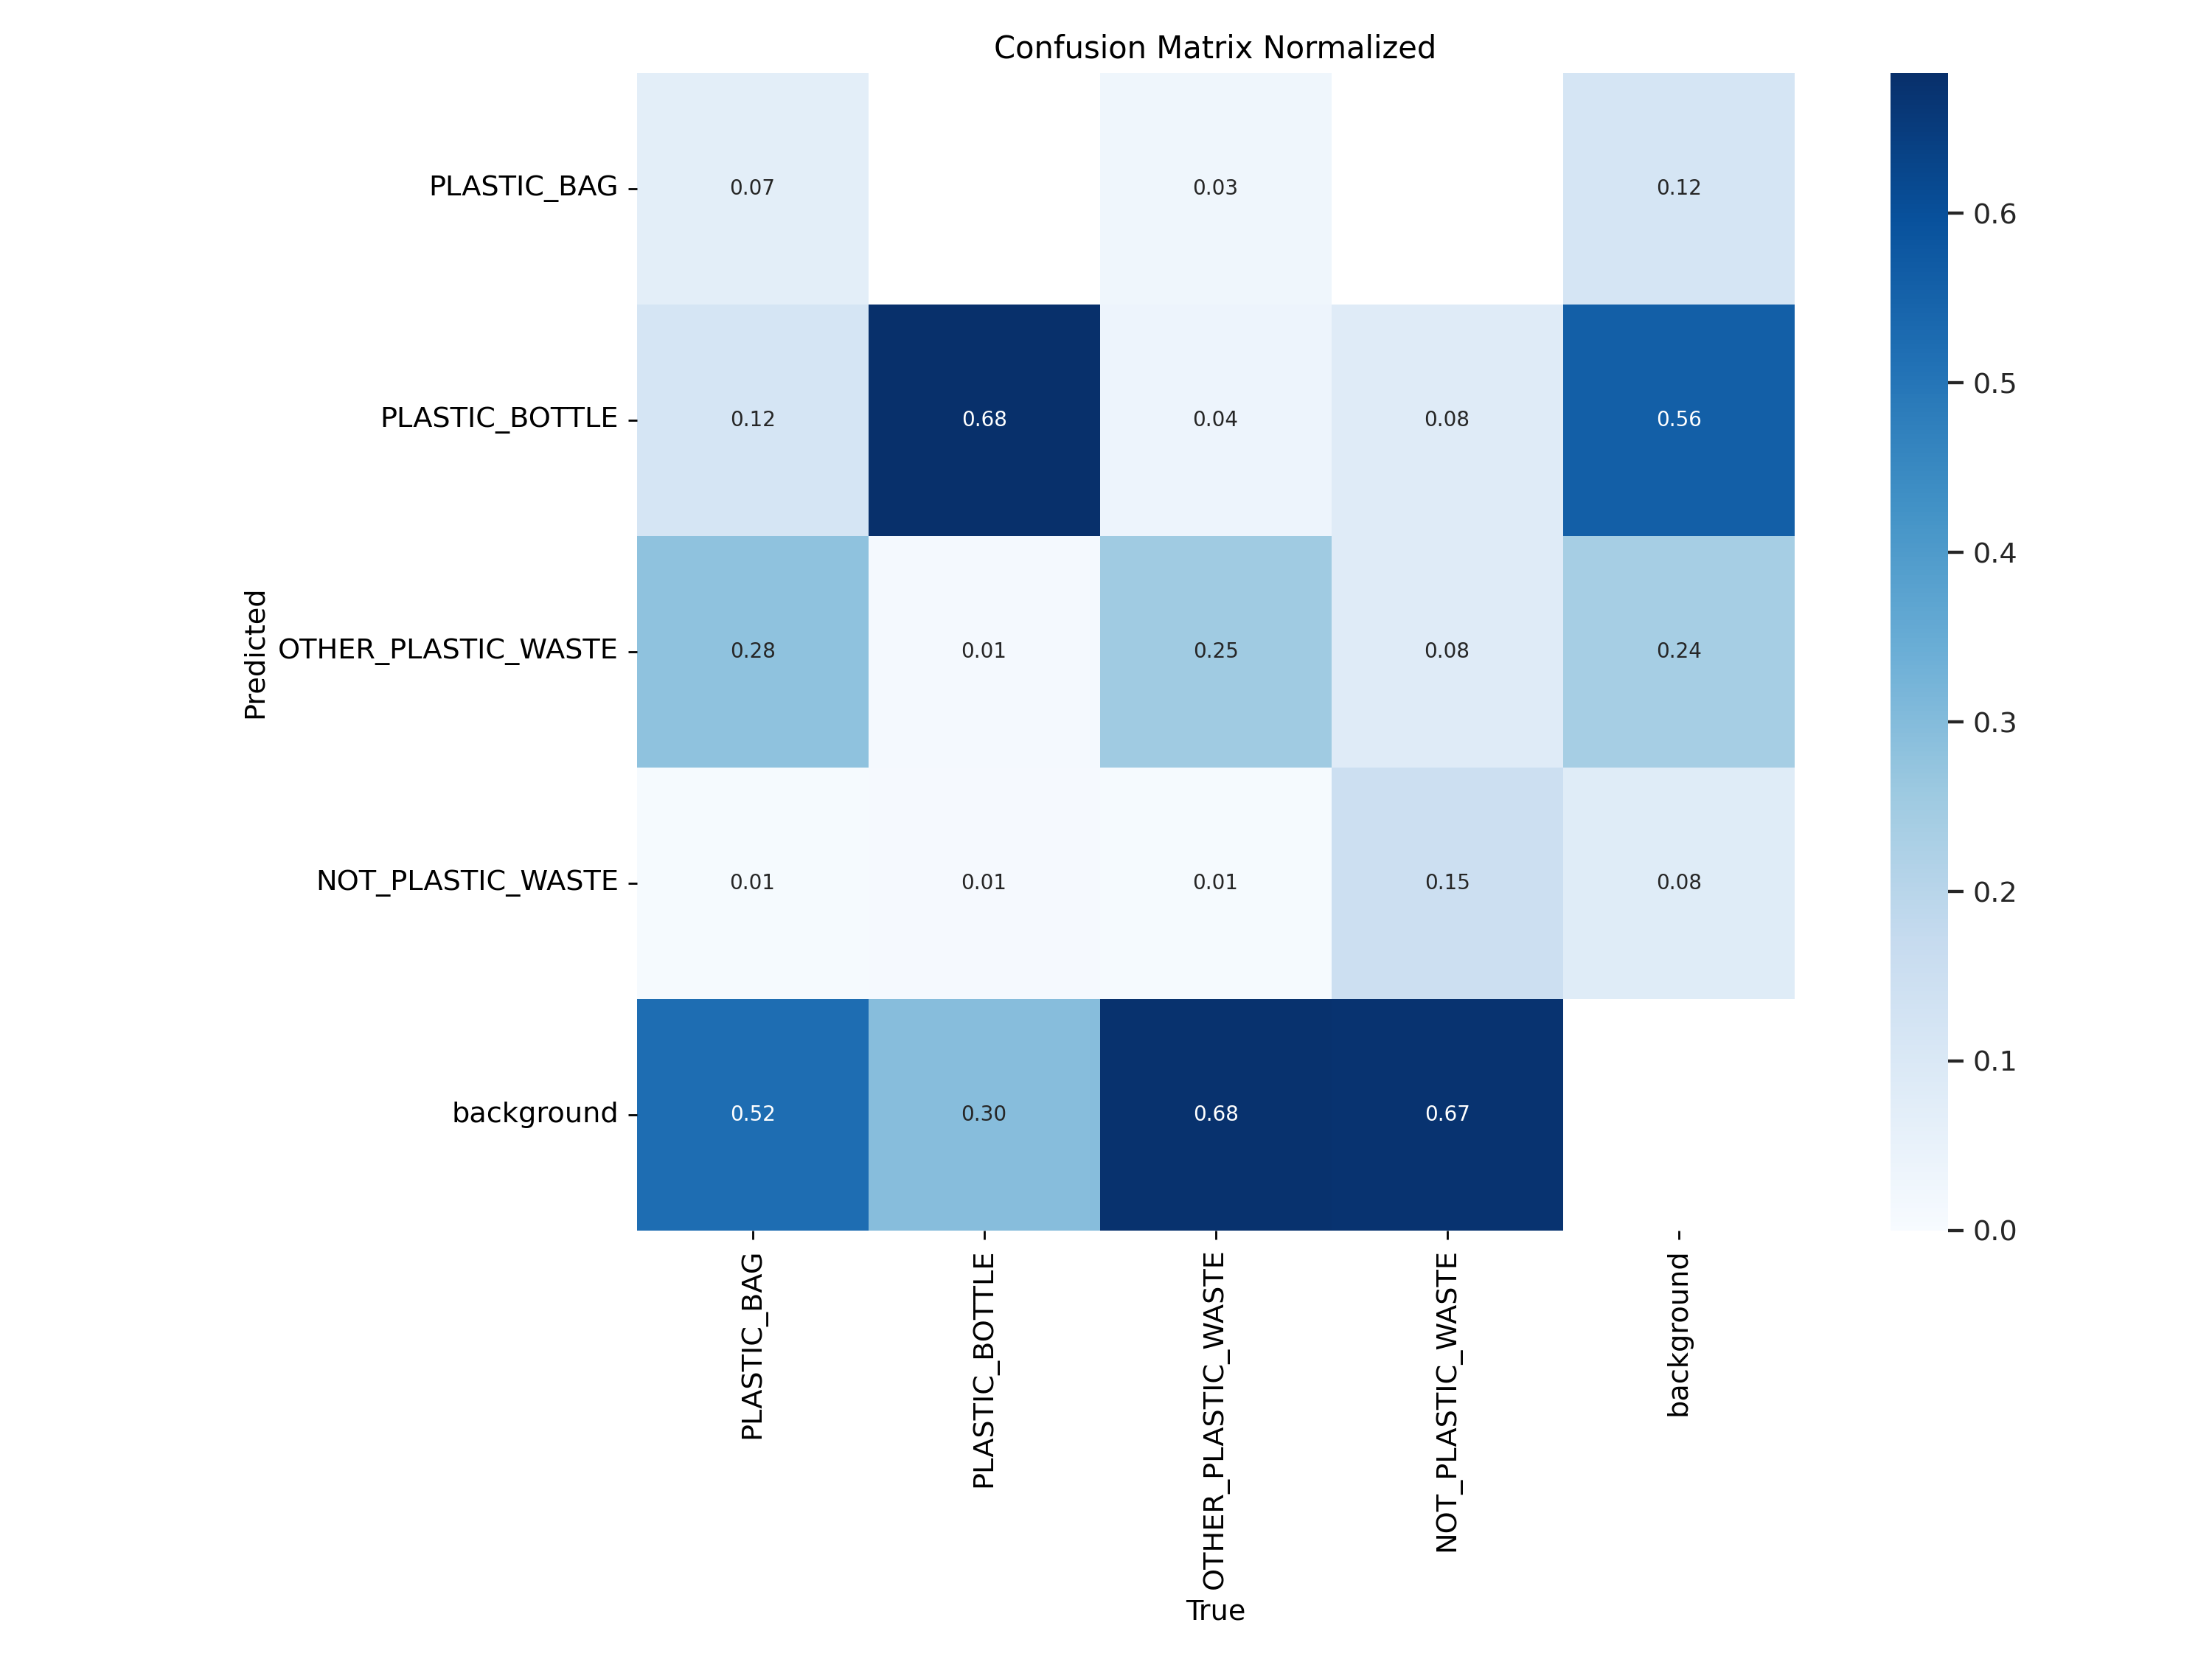
\includegraphics[width=0.8\textwidth]{v_3/confusion_matrix_normalized.png}
        \caption{Matrice di confusione normalizzata data dal modello \texttt{medium-200-0}}
        \label{fig:v3-4}
    \end{figure}
    % - tabella performance test set

